\documentclass[unicode,11pt,a4paper,oneside,numbers=endperiod,openany]{scrartcl}

\renewcommand{\thesubsection}{\thesection.\arabic{subsection}}

\usepackage{amssymb} % for \mathbb
\usepackage{listings}
\usepackage{xcolor}
\usepackage{amsmath}  % for align environment
\usepackage{graphicx}
\usepackage{float}

\restylefloat{figure}

\setlength{\parindent}{0pt}


\lstdefinestyle{matlab}{
    language=Matlab,
    basicstyle=\ttfamily\small,
    commentstyle=\color[RGB]{34,139,34},
    keywordstyle=\color[RGB]{0,0,255},
    numberstyle=\tiny\color[RGB]{128,128,128},
    numbers=left,
    stepnumber=1,
    frame=single,
    breaklines=true,
    backgroundcolor=\color[RGB]{240,240,240},
    tabsize=2,
    columns=flexible,
    showstringspaces=false
}

\usepackage{ifthen}
\usepackage[utf8]{inputenc}
\usepackage{graphics}
\usepackage{graphicx}
\usepackage{hyperref}

\pagestyle{plain}
\voffset -5mm
\oddsidemargin  0mm
\evensidemargin -11mm
\marginparwidth 2cm
\marginparsep 0pt
\topmargin 0mm
\headheight 0pt
\headsep 0pt
\topskip 0pt        
\textheight 255mm
\textwidth 165mm

\newcommand{\duedate} {}
\newcommand{\setduedate}[1]{%
\renewcommand\duedate {\textbf{Due date:}~ #1}}
\newcommand\isassignment {false}
\newcommand{\setassignment}{\renewcommand\isassignment {true}}
\newcommand{\ifassignment}[1]{\ifthenelse{\boolean{\isassignment}}{#1}{}}
\newcommand{\ifnotassignment}[1]{\ifthenelse{\boolean{\isassignment}}{}{#1}}

\newcommand{\assignmentpolicy}{
\begin{table}[h]
\begin{center}
\scalebox{0.8} {%
\begin{tabular}{|p{0.02cm}p{16cm}|}
\hline
&\\
\multicolumn{2}{|c|}{\Large\textbf{Numerical Computing 2023 ---  Submission Instructions}}\\
\multicolumn{2}{|c|}{\large\textbf{(Please, notice that following instructions are mandatory: }}\\
\multicolumn{2}{|c|}{\large\textbf{submissions that don't comply with, won't be considered)}}\\
&\\
\textbullet & Assignments must be submitted to \href{https://www.icorsi.ch/course/view.php?id=14666}{iCorsi} (i.e. in electronic format).\\
\textbullet & Provide both executable package and sources (e.g. C/C++ files, MATLAB). 
If you are using libraries, please add them in the file. Sources must be organized in directories called:\\
\multicolumn{2}{|c|}{\textit{Project\_number\_lastname\_firstname}}\\
& and  the  file must be called:\\
\multicolumn{2}{|c|}{\textit{project\_number\_lastname\_firstname.zip}}\\
\multicolumn{2}{|c|}{\textit{project\_number\_lastname\_firstname.pdf}}\\
\textbullet &  The TAs will grade your project by reviewing your project write-up, and looking at the implementation you attempted, and benchmarking your code's performance.\\

\textbullet & You are allowed to discuss all questions with anyone you like; however: (i) your submission must list anyone you discussed problems with and (ii) you must write up your submission independently.\\
\hline
\end{tabular}
}
\end{center}
\end{table}
}
\newcommand{\punkte}[1]{\hspace{1ex}\emph{\mdseries\hfill(#1~\ifcase#1{Points}\or{Points}\else{Points}\fi)}}


\newcommand\serieheader[6]{
\thispagestyle{empty}%
\begin{flushleft}

\includegraphics[width=0.45\textwidth]{CI_logo}
\end{flushleft}
  \noindent%
  {\large\ignorespaces{\textbf{#1}}\hspace{\fill}\ignorespaces{ \textbf{#2}}}\\ \\%
  {\large\ignorespaces #3 \hspace{\fill}\ignorespaces #4}\\
  \noindent%
  \bigskip
  \hrule\par\bigskip\noindent%
  \bigskip {\ignorespaces {\Large{\textbf{#5}}}
  \hspace{\fill}\ignorespaces \large \ifthenelse{\boolean{\isassignment}}{\duedate}{#6}}
  \hrule\par\bigskip\noindent%  \linebreak
 }

\makeatletter
\def\enumerateMod{\ifnum \@enumdepth >3 \@toodeep\else
      \advance\@enumdepth \@ne
      \edef\@enumctr{enum\romannumeral\the\@enumdepth}\list
      {\csname label\@enumctr\endcsname}{\usecounter
        {\@enumctr}%%%? the following differs from "enumerate"
	\topsep0pt%
	\partopsep0pt%
	\itemsep0pt%
	\def\makelabel##1{\hss\llap{##1}}}\fi}
\let\endenumerateMod =\endlist
\makeatother




\usepackage{textcomp}





\begin{document}


\setassignment
\setduedate{Wednesday, 6 December 2023, 11:59 PM}

\serieheader{Numerical Computing}{2023}{\textbf{Student:} Harkeerat Singh Sawhney}{}
\newline

\assignmentpolicy


\newpage

\section{General Questions [10 points]}

\subsection{Size of Matrix A}
From the Background Information given for this Project we do know that $A \in \mathbb{R}^{n^2 \times n^2} $ indicates the transformation matrix coming from the repeated application of what is referred to as the "image kernel", which in our case tends to produce the blurring effect. In the other hand $B$ is the transformed blurred image and $X$ is the original square, grayscale image matrix, in which each matrix entry corresponds to one pixel value. Hence the blurring computation can be defined be following equation:

\begin{equation}
    Ax = b
\end{equation}

In the above equation $x$ and $b$ are the vectorized repersentation of $X$ and $B$ respectively.

\begin{lstlisting}[style=matlab, caption={Computing the size of A}, label={lst:computing_size_of_A}]
    %% Load Default Img Data
    load('blur_data/B.mat');
    B=double(B);
    n = size(B,1);
    sizeA = n * n;
    disp(['Size of A: ', num2str(sizeA)]);
\end{lstlisting}

From the Code Listing \ref{lst:computing_size_of_A} we can see that the size of $A$ is $62500 \times 62500$. This is computed through the size of $B$ which is $250 \times 250$ and then multiplying it by itself.

\subsection{How many diagonal bands does A have?}
It is understood that A is a $d^2$-banded symmetric matrix, where $d << n$. Since we know that the size of the kernel image matrix is $7 \times 7$ then we can also compute the amount of diagonal bands that A has. Hence the amount of diagonal bands that A has is $49$.

\subsection{What is the length of the vectorized blurred image b}
In order to compute the length of the vectorized blurred image $b$, we need to compute the size of $B$ and then multiply it by itself. We know that $B$ is a $250 \times 250$ matrix, hence the length of the vectorized blurred image $b$ is $62500$.

\section{Properties of A [10 points]}
\subsection{If A is not symmetric, how would this affect $\tilde{A}$?}
A is used to compute the Conjugate Gradient method, which is an iterative method to solve the linear system $Ax = b$. If A is symmetric of full rank but not positive-definite we can bypass this issue by solving the augmented System.

\begin{align}
    A^TAx      & = A^Tb      \\
    \tilde{A}x & = \tilde{b}
\end{align}

In the above equation the pre-multiplication with $A^T$ ensures that the resulting matrix $\tilde{A}$ is symmetric and positive-definite. Hence even if A is not symmetric, we can still compute $\tilde{A}$ because of the properties of $A^T$.

\subsection{Explain why solving $Ax = b$ for $x$ is equivalent to minimizing $\frac{1}{2} x^T Ax - b^Tx$ over $x$, assuming that $A$ is symmetric positive\textendash definite.}

We want to show that by minimizing $\frac{1}{2} x^T Ax - b^Tx$ over $x$ is equivalent to solving $Ax = b$. We can do this by taking the derivative of $\frac{1}{2} x^T Ax - b^Tx$ with respect to $x$ and setting it to zero. Hence we get the following equation:

\begin{align}
    \frac{d}{dx} \left( \frac{1}{2} x^T Ax - b^Tx \right) & = 0                           \\
    \frac{1}{2} \left( x^T A + x^T A^T \right) - b^T      & = 0                           \\
    x^T A - b^T                                           & = 0                           \\
    x^T A                                                 & = b^T                         \\
    x^T                                                   & = b^T A^{-1}                  \\
    x                                                     & = \left( b^T A^{-1} \right)^T \\
    x                                                     & = \left( A^{-1} \right)^T b   \\
    x                                                     & = A^{-1} b                    \\
    Ax                                                    & = b
\end{align}

Hence can see at the end that we get the equation $Ax = b$ which is what we wanted to show.

\section{Conjugate Gradient [30 points]}

\subsection{Write a function for the conjugate gradient solver [x,rvec]=myCG(A,b,x0,max itr,tol), where x and rvecare, respectively, the solution value and a vector containing the residual at every iteration.}

In this question we are asked to write a function for the conjugate gradient solver. The function is called \texttt{myCG} and it takes in the following parameters: \texttt{A}, \texttt{b}, \texttt{x0}, \texttt{max\_itr} and \texttt{tol}. The function returns the solution value \texttt{x} and a vector containing the residual at every iteration \texttt{rvec}. The function is implemented in the Code Listing \ref{lst:myCG}. The code is written from the provided Conjugate Gradient Algorithm in the Project Description.
\\
\\
The function first initializes the solution $x$ with the initial guess $x0$, and computes the initial residual $r$ as $b - A * x0$. the direction $d$ is also initialized as r. Then the function enters a for loop which iterates for the maximum number of iterations. In each iteration, it performs the steps which is provided in the algorithm.

\begin{lstlisting}[style=matlab, caption={Matlab function for Conjugate Gradient}, label={lst:myCG}]
    function [x, rvec] = myCG(A, b, x0, maxIter, tol)
        rvec = [];	
        x = x0;
        r = b - A * x0;
        d = r;
        pho_old = dot(r, r);
        
        
        for i = 1:maxIter
            s = A * d;
            alpha = pho_old / dot(d, s);
            x = x + alpha * d;
            r = r - alpha * s;
            pho_new = dot(r, r);

            beta = pho_new / pho_old;
            d = r + beta * d;
            pho_old = pho_new;
            
            rvec = [rvec, pho_new];

            if sqrt(pho_new) < tol
                disp('Converged');
                break;
            end
            
            
        end
    end
\end{lstlisting}

\subsection{In order to validate your implementation, solve the system defined by A test.matand b test.mat. Plot the convergence (residual vs iteration)}

\begin{figure}[H]
    \centering
    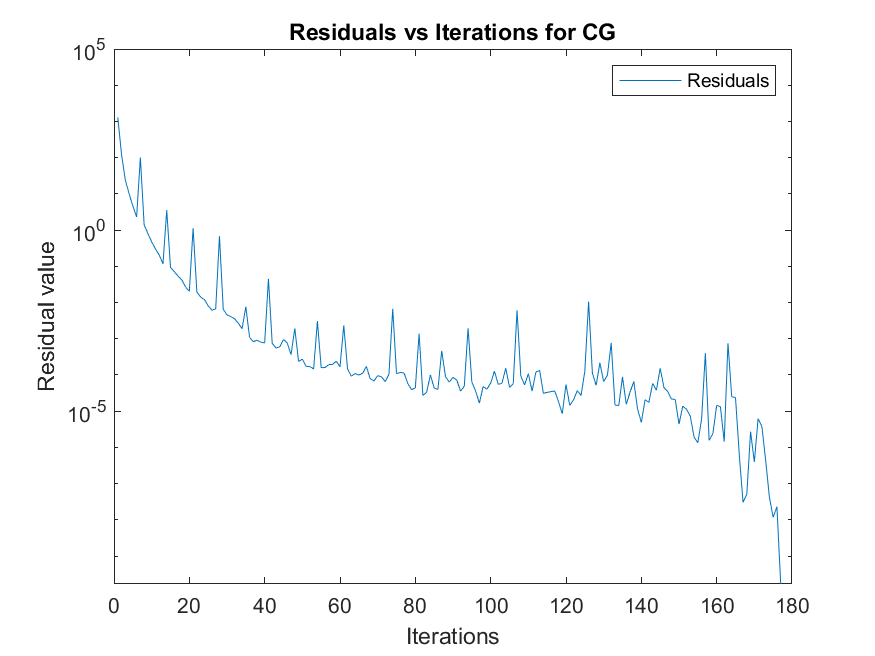
\includegraphics[width=0.8\linewidth]{graphs/residuals.png}
    \caption{Residuals vs Iterations for the Conjugate Gradient Algorithm}
    \label{fig:residuals}
\end{figure}

In this question we are asked to validate our implementation of the Conjugate Gradient Algorithm. We are given the matrix $A$ and the vector $b$. We are then asked to use the function which we implemented in the previous question to solve the system $Ax = b$. When we obtain the solution $x$ we are asked to plot the convergence of the residuals vs the iterations. The plot is shown in Figure \ref{fig:residuals}.

Our maximum number of iterations is set to 200 and the tolerance is set to $10^{-4}$. From the Figure \ref{fig:residuals} we can see that the residuals converge right before the 180th iteration. Also the from the plot we can see that the residual overall decreases, but does has multiple spikes in between.

\subsection{Plot the eigenvalues of A test.matand comment on the condition number and convergence rate.}
In this question we are asked to plot the eigenvalues of $A$ and comment on the condition number and the convergence rate. Condition Number is defined as the ratio of the largest eigenvalue to the smallest eigenvalue. The condition number $\kappa(A)$ is the relation of sensitivy of the solution $x$ to the changes in the right hand side $b$. The condition number is computed as follows:

\begin{equation}
    \kappa(A) = \frac{\lambda_{max}}{\lambda_{min}}
\end{equation}

If small changes in $b$ cause large changes in $x$, then the system is called as ill-conditioned and the condition number of the system is large. However if small changes in $b$ cause small changes in $x$, then the system is called as well-conditioned and the condition number of the system is small. Hence the condition number is a measure of the sensitivity of the solution $x$ to the changes in the right hand side $b$.

Hence in order to compute the condition number of $A$ we need to compute the eigenvalues of $A$. The eigenvalues of $A$ are computed using the \texttt{eig} function in Matlab. The eigenvalues are then sorted in ascending order and plotted. The plot is shown in Figure \ref{fig:eigenvalues}. As it can be seen in the plot the difference between the largest eigenvalue and the smallest eigenvalue is very large. Hence the condition number of $A$ is very large. This means that the system is ill-conditioned and small changes in $b$ will cause large changes in $x$. This can also be seen by calculating the condition number of $A$. We can do that by using the inbuilt \texttt{cond} function in Matlab. The condition number of $A$ is approximately $1.67 \times 10^{6}$ which is very large. Hence this is aligned with our previous observation that the system is ill-conditioned.



\begin{figure}[H]
    \centering
    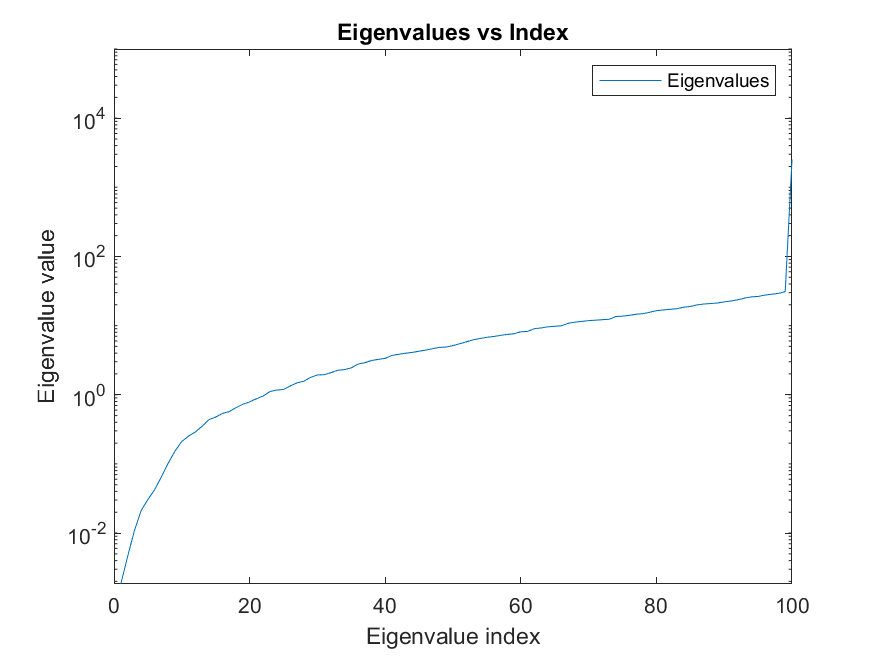
\includegraphics[width=0.8\linewidth]{graphs/eigenvalues.png}
    \caption{Eigenvalues of A}
    \label{fig:eigenvalues}
\end{figure}

\subsection{Does the residual decrease monotonically? Why or why not?}
As it can be seen from Figure \ref{fig:residuals} the residual does not decrease monotonically. The residual decreases overall but has multiple spikes in between. Therefore when we are computing the residuals, we are computing the difference between the actual solution $x$ and the computed solution $x$. Since the system is ill-conditioned, small changes in $b$ will cause large changes in $x$. Hence the residual will have multiple spikes in between, but will overall decrease.


\section{Deblurring problem [35 points]}



\end{document}
